\documentclass[conference]{IEEEtran}
\usepackage{graphicx}
\usepackage{booktabs}
\usepackage{amsmath}
\usepackage{url}
\usepackage[hidelinks]{hyperref}
\renewcommand{\ttdefault}{cmtt}

\title{Serialization Order Confounds Attention Analysis in MeshXL}

\author{\IEEEauthorblockN{Minu Choi}
\IEEEauthorblockA{School of Data Science\\
University of Virginia\\
Charlottesville, VA\\
qce2dp@virginia.edu}}

\begin{document}
\maketitle

\begin{abstract}
Autoregressive mesh transformers look like an unusually convenient target for
mechanistic interpretability: the token stream \emph{is} the geometry, so every
attention weight has a literal spatial address and can be painted onto the
surface being generated. We show that this convenience is a trap. In MeshXL's
canonical serialization, faces arrive sorted by height, so a face's index in the
token stream predicts its vertical position at Spearman $\rho = 0.951$ across all
2820 training chairs, and a cubic in normalized sequence position explains 86\%
of height variance. Any attention map read spatially is therefore confounded with
plain recency. The confound is structural rather than incidental: it is a
property of the preprocessing, its median across four object categories ranges
only from $+0.914$ to $+0.968$, and re-ordering faces to break it raises
cross-entropy fortyfold on every mesh tested. Controlling for sequence position
on unmodified inputs, attention's partial correlation with 3D proximity is
$+0.194$ (95\% CI $[+0.165, +0.206]$) against $+0.430$ for sequence proximity;
the spatial estimate replicates at $+0.180$ ($[+0.167, +0.199]$) on a disjoint
held-out sample. No head in the network is primarily geometric, none reaching
$\rho_{\text{spatial}} = 0.50$ while $\rho_{\text{seq}}$ reaches $+0.951$, and
layers 0--11 carry no geometric selectivity at all. Testing mesh topology, a
geometric feature nearly independent of the confound, attention does not track it
($+0.041$, no head above $+0.15$), while sensitivity to repeated coordinate
tokens between non-touching faces is twice as strong. Separately, MeshXL inherits
OPT-1.3b's transformer body and reinitializes only its embeddings; we find its
attention sinks bear no relation to OPT's ($\rho = -0.146$) while being sevenfold
stronger, so they form under mesh training rather than arriving with the weights.
All confirmatory claims follow rules fixed before any attention was extracted.
Of three such arms, one returned inconclusive, one failed its own validity gate,
and one was refuted; all three are reported as they landed.
\end{abstract}

\section{Introduction}

Mechanistic interpretability has developed a toolkit around language models, and
a recurring question is how much of it transfers to other modalities.
Autoregressive mesh generators look like an inviting place to ask. MeshXL
\cite{chen2024meshxl}, following PolyGen \cite{nash2020polygen} and MeshGPT
\cite{siddiqui2024meshgpt}, emits a 3D mesh as a flat sequence of quantized
coordinates: nine tokens per triangle, three vertices of three coordinates each.
Unlike a language model, where the relationship between a token and any
real-world referent is opaque, here the sequence \emph{is} the object. Every key
position corresponds to a specific triangle at a specific place in space, so
attention can be rendered directly onto the mesh surface and read off by eye.

That affordance is what makes the domain attractive, and it is also what makes it
dangerous. A picture of attention concentrated on the legs of a chair is
persuasive in a way a bar chart over token indices is not, and persuasive
pictures invite conclusions the underlying statistic does not support.

This paper is an audit of what such pictures actually show. Our central finding
is methodological: in the canonical serialization these models are trained on, a
face's position in the token sequence and its height in space are very nearly the
same variable. Attention that is merely recent will therefore look spatially
organized, and organized along the sort axis. We quantify the confound, show it
cannot be removed by the obvious interventions, and then measure what survives
once it is controlled.

Our contributions are:

\begin{enumerate}
\item We identify and quantify a structural confound between sequence position
and vertical position in mesh transformer serializations
(Section~\ref{sec:confound}), and show it is a property of preprocessing rather
than of the data, holding uniformly across four object categories.
\item We measure attention's partial association with 3D proximity while
controlling for sequence distance, on unmodified inputs, and replicate it on a
held-out sample (Section~\ref{sec:e1}).
\item We show that re-ordering faces to break the confound destroys the model,
which both rules out that intervention and constitutes independent evidence that
the model represents the sequence rather than the shape (Section~\ref{sec:e2}).
\item We test mesh topology, a geometric feature nearly independent of the
confound, and find it is not tracked, while sensitivity to repeated coordinate
tokens is twice as strong (Section~\ref{sec:e4}).
\item We exploit the fact that MeshXL inherits OPT's weights to ask whether
attention sinks survive a modality transplant, a comparison the language-only
literature cannot construct (Section~\ref{sec:e3}).
\end{enumerate}

All confirmatory analyses were preregistered with interpretation rules fixed in
advance. Code, preregistrations with results appended, and run artifacts are
available.\footnote{\url{https://github.com/minuuva/meshlens}, archived at
\url{https://doi.org/10.5281/zenodo.22149960}}

\section{Related Work}

\textbf{Attention sinks.} Transformers routinely allocate large attention mass to
a small number of positions, typically the first, that carry little information
\cite{xiao2023streamingllm}. Barbero et al. \cite{barbero2025active} characterize
heads as active or dormant by how much of their attention goes to such sinks. Gu
et al. \cite{gu2025attention} attribute sink formation to softmax normalization
together with the loss and data distribution, and leave open how much is
architectural. Testing that cleanly would require the same transformer body
trained on a different modality, which is difficult to arrange deliberately;
Section~\ref{sec:e3} exploits a case where it happened by accident.

\textbf{Ground-truth testbeds.} A persistent obstacle in interpretability is that
the true features of a model are unknown, which is why synthetic domains with
known state have become standard evaluation grounds
\cite{li2023emergent,karvonen2024measuring}. Karvonen et al.
\cite{karvonen2024measuring} note that such testbeds remain ``confined to the
chess and Othello domains,'' and that comparable objective metrics for other
domains remain a significant challenge. Mesh transformers are appealing partly
for this reason: coordinate slot, coordinate value, face membership, and mesh
topology are all exactly known from the data, with no annotation. Our results
temper that appeal by showing how much of the apparent structure in this domain
is an artifact of how the ground truth is ordered.

\textbf{Attention as evidence.} Attention weight is not causal contribution, and
gradient-weighted variants exist precisely because raw attention overclaims
\cite{barkan2021gradsam,jiang2025devils}. Our argument is upstream of that
critique: even as a purely descriptive statistic about where a head looks,
attention in this domain is confounded before any causal question is asked.

\section{The Confound}
\label{sec:confound}

MeshXL's tokenizer performs no sorting. It gathers face coordinates in the order
the data already has and flattens them to nine tokens per face, so a face's index
in the stored array is exactly its position in the token stream. The ordering is
imposed earlier, during preprocessing, which sorts faces by coordinate.

The consequence is severe. Fig.~\ref{fig:confound} shows the Spearman correlation
between face index and each centroid coordinate, computed on every one of the
2820 training chairs with at least 50 faces. The vertical axis correlates at
$+0.935$ mean and $+0.951$ median, with 82\% of chairs above $0.9$; the other two
axes sit at $+0.097$ and $-0.277$. A cubic in normalized sequence position
explains 86\% of height variance on average.

\begin{figure*}[t]
\centering
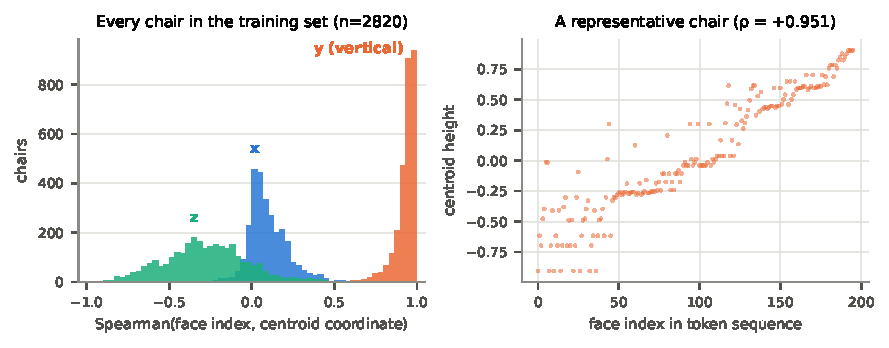
\includegraphics[width=\textwidth]{figures/confound.pdf}
\caption{Face index and vertical position are very nearly the same variable.
Left: the distribution over all 2820 training chairs, per axis. Right: one
representative chair. A claim that early layers attend to chair legs and late
layers to chair backs is not separable from plain recency under this ordering.}
\label{fig:confound}
\end{figure*}

This is not a property of chairs. Across all four categories MeshXL's supervised
fine-tunes cover, the median correlation between face index and height ranges
only from $+0.914$ to $+0.968$ (Table~\ref{tab:categories}). Every mesh in every
category is sorted the same way, because the sort belongs to the preprocessing
rather than to the object. There is consequently no subset of the data, and no
choice of category, in which the confound is materially weaker.

\begin{table}[t]
\centering
\caption{The confound is uniform across object categories. $R^2$ is for a cubic
fit of centroid height on normalized sequence position.}
\label{tab:categories}
\begin{tabular}{lrrr}
\toprule
category & meshes & $\rho$(index, height) & $R^2$ \\
\midrule
chair & 2820 & $+0.951$ & 0.858 \\
table & 4632 & $+0.914$ & 0.778 \\
lamp  & 564  & $+0.968$ & 0.844 \\
bench & 504  & $+0.939$ & 0.826 \\
\bottomrule
\end{tabular}
\end{table}

Some room remains: 36\% of the height standard deviation survives that cubic fit,
and over causal face pairs, sequence distance and 3D distance share only about a
third of their variance (Spearman $+0.569$). The effect is therefore separable in
principle. It has to be separated deliberately rather than assumed away, which is
what the rest of this paper does.

\section{Methodology}

\subsection{Model and Data}

All experiments use MeshXL-1.3b fine-tuned on ShapeNet chairs (category 03001627)
\cite{zhang2023shapenet}: an OPT decoder with 24 layers, 32 heads, and hidden
dimension 2048, over a vocabulary of 131 tokens (128 coordinate bins plus BOS,
EOS, PAD). Attention is read teacher-forced, one forward pass per mesh.

Two implementation details matter for reproduction. MeshXL's constructor calls
\texttt{to\_bettertransformer()}, which installs a fused attention kernel that
never materializes the softmax matrix; attention weights cannot be read through
it, and we force an eager implementation instead. And MeshXL's inverse
discretization is $(t + 0.5)/128 \times 2 - 1$, not $t/127 \times 2 - 1$; the two
are affine in $t$, so correlations are unaffected, but absolute distances are not.

\subsection{Definitions}

Face-level attention $a(q,k)$ is the mean of the $9\times 9$ token block from face
$q$'s query rows onto face $k$'s key columns, with the sink region (BOS and face
0) excluded and each row renormalized over its causal non-sink keys. A head is
\emph{dormant} when its mean sink attention over the final face's query rows
exceeds $0.5$, and \emph{active} otherwise. Only pairs with $k < q$ enter any
statistic.

\subsection{Estimator}

All partial correlations are Spearman, computed per chair and then aggregated,
with confidence intervals bootstrapped over chairs (1000 resamples). Pair count
grows with the square of face count, so pooling raw pairs across a sample
spanning 50 to 800 faces would weight the largest meshes some 250 times more
heavily than the smallest.

\subsection{Preregistration}

Each confirmatory experiment has an interpretation rule fixed before any
attention was extracted, together with the sample, the head classification, and
the thresholds. Samples are two disjoint 100-chair splits drawn from a single
seeded permutation. We report inconclusive results as inconclusive; no threshold
was adjusted after the fact.

\section{Results}

\subsection{Attention is Predominantly Recency}
\label{sec:e1}

On unmodified, canonically ordered meshes we compute, for each head, the partial
Spearman correlation of face attention with 3D proximity controlling for sequence
distance ($\rho_{\text{spatial}}$), and with sequence proximity controlling for 3D
distance ($\rho_{\text{seq}}$). This is a zero-intervention measurement: the model
sees exactly the inputs it was trained on.

At the final layer, across 19 active heads and 100 chairs,
$\rho_{\text{spatial}} = +0.194$ (95\% CI $[+0.165, +0.206]$) against
$\rho_{\text{seq}} = +0.430$ ($[+0.412, +0.472]$). The preregistered rule required
$\rho_{\text{spatial}} \geq 0.20$ with an interval excluding zero to support
spatial selectivity; the estimate falls six thousandths short, and the verdict is
inconclusive.

An inconclusive verdict is ambiguous between a sample too small and an effect that
genuinely lies between the thresholds, and those call for opposite responses. The
held-out split resolves it: $\rho_{\text{spatial}} = +0.180$ ($[+0.167, +0.199]$),
overlapping and inconclusive on its own terms. Two independent samples of 100
chairs estimating $0.194$ and $0.180$ with intervals of width $0.04$ describe a
real, reproducible, and modest effect of about $0.19$. Additional data would
narrow the interval without moving it. We report the splits separately and do not
pool them.

\begin{figure*}[t]
\centering
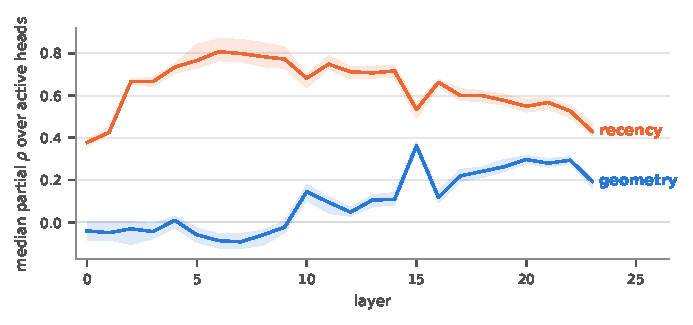
\includegraphics[width=0.78\textwidth]{figures/layer_profile.pdf}
\caption{Recency dominates at every depth. Geometry is absent or slightly negative
through layer 9 and emerges only in the second half of the network, which inverts
the usual reading of layer-wise geometric specialization. Bands are bootstrap 95\%
intervals over chairs.}
\label{fig:layers}
\end{figure*}

The depth profile (Fig.~\ref{fig:layers}) is more informative than the single
primary statistic. Recency runs from $+0.38$ at layer 0 to a peak of $+0.81$ at
layer 6, and is still $+0.43$ at the output. Geometry is absent or slightly
negative through layer 9, turns positive around layer 10, and peaks near $+0.36$
at layer 15. Over active heads, layers 0--11 have median
$\rho_{\text{spatial}} = -0.043$, with 65 of 84 at or below zero; layers 12--23
have median $+0.260$, with 6 of 179 at or below zero.

This bears directly on claims of layer-wise geometric specialization. Under this
serialization, early layers attend to early tokens, and early tokens are low on
the object. Once sequence position is controlled, the early layers carry no
spatial selectivity whatsoever. The pattern that reads as ``legs first, backs
later'' is recency, and the mechanism runs opposite to the geometric story.

Across all 768 head slots, no head reaches $\rho_{\text{spatial}} = 0.50$; the
maximum anywhere is $+0.469$, while $\rho_{\text{seq}}$ reaches $+0.951$. Of the
263 active heads, 10 are more spatial than recency-driven. No head in this model
is primarily geometric, and Fig.~\ref{fig:taxonomy} shows why that is easy to
miss: heads do separate by depth and do occupy distinct positions, so a
head-by-head survey finds real structure. It is simply structure along the
recency axis.

\begin{figure}[t]
\centering
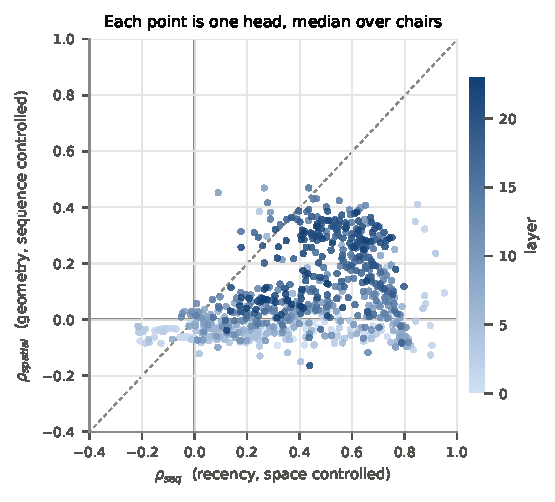
\includegraphics[width=\linewidth]{figures/head_taxonomy.pdf}
\caption{Every head, placed by what its attention tracks. Points below the
diagonal are more recency-driven than geometric. Early layers (light) form a band
at zero geometric selectivity spread across a wide range of recency; later layers
(dark) rise, but none crosses into primarily geometric territory.}
\label{fig:taxonomy}
\end{figure}

\subsection{Re-ordering Destroys the Model}
\label{sec:e2}

The obvious way to break the confound is to change the sort. Re-sorting faces
lexicographically with $x$ as the leading key moves the coupling cleanly: index
versus height falls from $+0.953$ to $+0.015$ while index versus $x$ reaches
$+1.000$, and the mesh remains a sorted mesh of exactly the same geometry, with
only presentation order changed.

The model does not tolerate it. Cross-entropy rises from $0.055$ to $2.203$, a
factor of forty, on every one of 37 chairs measured, with a median per-chair ratio
of $49\times$ and a minimum of $12\times$ (Fig.~\ref{fig:gate}). Our preregistered
validity gate treats any ratio above $2\times$ as evidence that the input is too
far off-distribution to support conclusions about head function, so we report no
head-level statistics from this arm.

\begin{figure*}[t]
\centering
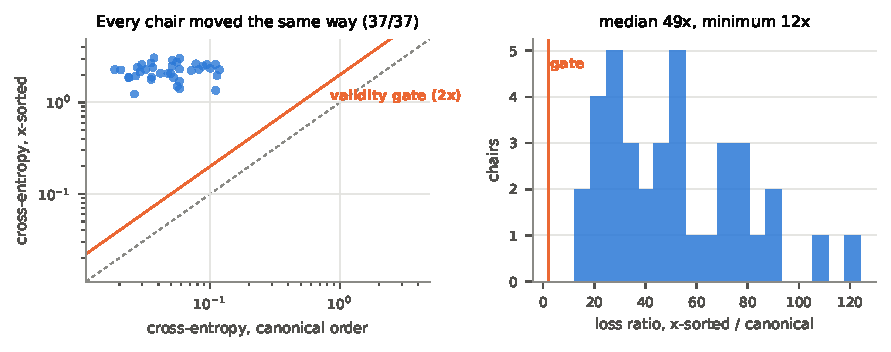
\includegraphics[width=\textwidth]{figures/validity_gate.pdf}
\caption{Re-ordering faces changes no geometry, only presentation order, and costs
a fortyfold rise in cross-entropy. Log axes; the dashed line is no change.}
\label{fig:gate}
\end{figure*}

Two things follow. First, the confound is not breakable by reordering, and a
random shuffle would fare worse than a re-sort rather than better, so that avenue
is closed. Second, the measurement is informative in its own right. A model
representing the shape should be substantially indifferent to the order in which
that shape is presented. This one is not, which is independent evidence for the
same conclusion Section~\ref{sec:e1} points toward and does not depend on where
the threshold in that section was placed.

\subsection{Topology is Not Tracked; Token Repetition Is}
\label{sec:e4}

Metric proximity is entangled with the confound at $+0.569$, which limits how
sharply Section~\ref{sec:e1} can speak. Mesh topology is not. Two faces sharing an
edge is exact ground truth shipped with the data, requiring no threshold and no
metric choice, and it is nearly independent of the nuisance: adjacency correlates
$-0.153$ with sequence distance and $-0.165$ with 3D distance, and 52\% of
adjacent pairs are more than three positions apart in the token stream. It is also
the property a mesh generator would most plainly need in order to close a surface.

On the held-out 100 chairs we compute $\rho_{\text{adj}}$, the partial correlation
of attention with adjacency controlling for \emph{both} sequence distance and 3D
distance. At the final layer it is $+0.041$ (95\% CI $[+0.037, +0.044]$). The
preregistered rule calls this refuted: attention carries no topological structure
once recency and proximity are accounted for. No head anywhere in the network
exceeds the $+0.15$ band, and the maximum is $+0.074$.

The intended control is more interesting than the primary. Adjacent faces share
two vertices and therefore six of eighteen coordinate tokens, so an apparent
topological effect might be token matching. We measure that directly as
$\rho_{\text{shared}}$, the same partial correlation against the number of shared
vertex positions, computed over \emph{non-adjacent} pairs only. It is $+0.086$
($[+0.082, +0.093]$): twice the adjacency effect. Over all 261 active head slots,
shared-token sensitivity exceeds adjacency in 93.5\% of them, with medians of
$+0.095$ against $+0.047$, and the ordering holds in all 24 layers. Ten heads
clear $+0.15$ on shared tokens; none do on adjacency.

Because these pairs do not touch, this is not adjacency arriving under another
name. It is sensitivity to repeated coordinate \emph{values} between unrelated
faces, which is a lexical mechanism rather than a geometric one. What little
structure survives our controls looks like a model matching repeated tokens, as a
language model does, rather than one tracking the surface it is building.

\subsection{Sinks Do Not Survive a Modality Transplant}
\label{sec:e3}

MeshXL loads pretrained OPT weights and reinitializes only the word and positional
embeddings. The transformer body is therefore inherited across a complete change
of vocabulary and modality, and both models are OPT-1.3b shaped, which makes
per-head sink attention comparable cell by cell. This is the controlled comparison
the sink literature otherwise lacks.

Using the same sink definition for both, the first ten tokens read from the final
nine query rows, and matching lengths at OPT's native 2048-token context, the two
$24 \times 32$ grids are unrelated: Spearman $-0.146$ ($[-0.216, -0.078]$).
Knowing which heads sink in OPT tells one nothing about which heads sink in
MeshXL.

\begin{figure*}[t]
\centering
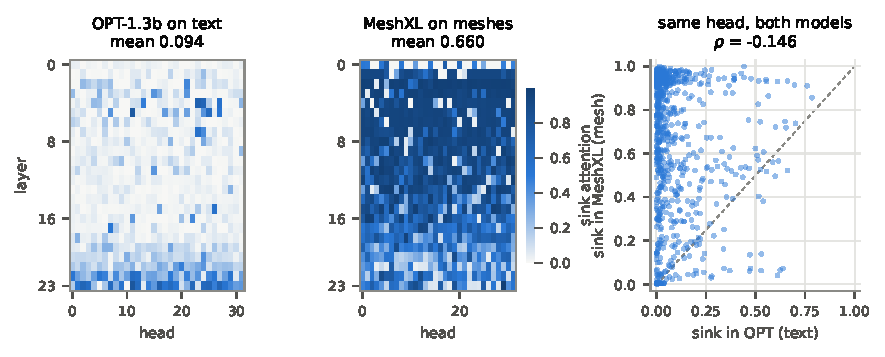
\includegraphics[width=\textwidth]{figures/sink_transfer.pdf}
\caption{Same transformer body, unrelated sink structure. MeshXL inherits
OPT-1.3b's weights and reinitializes only the embeddings, yet 72\% of its heads
sink above $0.5$ against 4\% of OPT's, and the per-head maps do not correspond.}
\label{fig:sink}
\end{figure*}

The magnitudes, which the rule did not cover, are the larger surprise
(Fig.~\ref{fig:sink}). MeshXL's mean sink attention is $0.660$ with 72\% of its
768 heads above $0.5$; OPT's is $0.094$ with 4\% above. The depth profiles are
close to inverted: MeshXL sinks hardest through layers 1--13 and relaxes toward
the output, while OPT stays low until layers 21--23. Whatever sink structure
MeshXL has, it formed under mesh training rather than arriving with the weights,
which supports a data-and-loss account of sink formation \cite{gu2025attention}
over an architectural one.

\section{Discussion}

The unifying observation is that this model behaves like a sequence model over a
canonically ordered stream, and much less like a model of three-dimensional shape.
Recency dominates its attention at every depth. Reordering a fixed shape costs it
most of its predictive power. It does not track which faces touch. The closest
thing to a positive geometric result, a partial correlation of about $0.19$ with
metric proximity, is real and replicable but modest, and confined to the second
half of the network.

For interpretability practice in this domain the implication is narrow and
concrete. Rendering attention onto a mesh surface is a compelling visualization
and a poor statistic. Under the standard serialization, any head attending to
recent tokens produces a picture that is spatially organized along the sort axis,
and that picture will look like structure. Reporting such maps without a recency
control is reporting the sort order.

The result also complicates the case for mesh transformers as ground-truth
interpretability testbeds. The appeal is that features like coordinate slot,
coordinate value, face membership, and topology are exactly known. That remains
true. But the canonical ordering couples the most salient of those features to
position so tightly, and the model depends on that ordering so heavily, that the
domain supplies known features and a built-in confound in the same package. A
testbed of this kind needs its nuisance structure characterized before its ground
truth is useful, which is a requirement the discrete board-game testbeds
\cite{li2023emergent,karvonen2024measuring} do not face, since position and state
are already decoupled there.

\section{Limitations}

Our measurements are correlational. We control statistically for sequence and
metric distance, and the one intervention we attempted failed its own validity
gate, so we make no causal claims about head function. Establishing those would
require activation patching, which we did not perform.

All results are from one model at one scale fine-tuned on one object category. The
confound generalizes across categories because it is a preprocessing property, but
the attention results may not.

The sink comparison in Section~\ref{sec:e3} sets a chair fine-tune against a base
model, so some of the difference may reflect fine-tuning rather than modality. Its
sink definition is symmetric by construction, but the first ten tokens constitute
a complete first triangle for a mesh and nine arbitrary words for text.

Experiment 2 was halted after 37 of its 100 preregistered chairs once the gate
outcome was beyond doubt; every chair had moved the same way and the smallest ratio
observed was six times the gate.

\section{Conclusion}

Attention in an autoregressive mesh transformer tracks the order in which the mesh
was serialized far more than the geometry of the mesh itself. The confound
responsible is structural, uniform across object categories, and not removable by
reordering, because the model's competence depends on the ordering. What survives
a proper control is a modest and replicable association with metric proximity,
confined to the network's second half, no association with mesh topology at all,
and a sensitivity to repeated coordinate tokens that is twice as strong as either.

We would emphasize the process as much as the findings. Of three confirmatory
arms, one returned inconclusive, one failed its validity gate, and one was
refuted. Fixing the rules in advance is what made those outcomes reportable rather
than embarrassing, and in the one case where the estimate fell six thousandths
short of a threshold, it is what kept the threshold where it was.

\bibliographystyle{IEEEtran}
\bibliography{references}

\end{document}
